\documentclass[9pt,addpoints]{exam}
\usepackage{enumitem}
\usepackage{amsfonts,amssymb,amsmath, amsthm}
\usepackage{graphicx}
\usepackage{systeme}
\usepackage{pgf,tikz,pgfplots}
\pgfplotsset{compat=1.15}
\usepgfplotslibrary{fillbetween}
\usepackage{mathrsfs}
\usetikzlibrary{arrows}
\usetikzlibrary{calc}
\pagestyle{headandfoot}
%\firstpageheadrule
\runningheader{Current}{}{Page \thepage\ of \numpages}
\runningheadrule
\author{Aaron GK}
\title{Magnetic Fields and Force}
\usepackage{geometry}
\geometry{
	a4paper,
	total={170mm,257mm},
	left=10mm,
	right=10mm,
	bottom=5mm,
	top=5mm,
}
\begin{document}
	\maketitle
	\subsection*{Force Fields}
	Early on in dynamics, we have seen that we can categorize forces as being \textbf{contact} or \textbf{non-contact} based on the need of contact in order for the force to be experienced. Non-contact forces act over distance and their pattern of action is determined by a \textbf{force field} - a region in which the non-contact force is exerted and felt.\newline\newline
	Common examples of non-contact forces include gravitation, magnetic force, and electric force. One thing common about them all? They all act over space(\textit{action at a distance}) and don't necessarily need contact in order to be felt. 
	\subsection*{Magnetic Fields}
	Magnetic Fields are no different from other non-contact forces in that they act over a distance. We have seen in Electrostatics that the \textit{Coulomb	Force} acts on the electric field. Electric Field is projected radially outwards from a positive charge and radially inwards in a negative charge. The source of any magnetic field possesses two poles, a \textbf{north pole} and a \textbf{south pole}. The poles received their names because of the way a magnet, such as that in a compass, behaves in the presence of the Earth’s magnetic field when suspended freely. \newline 
	As with positive charges, magnetic field lines come out of the north pole. Similar to negative charges, magnetic field lines go inside the south pole of a magnet. If we draw the magnetic field lines across a bar magnet, we can see the following pattern. \newline
	%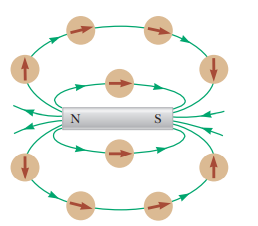
\includegraphics[scale=1.0]{img/magnetic_field_bar.png}\newline \newline
	The magnetic field lines outside a magnet start from the North Pole and go into the South, while inside the magnet it goes from the South to the North pole. It is a universal characteristic of all magnets that like poles repel and unlike poles attract, however, it is impossible to separate a magnetic pole on its own. \newline \newline
	\subsection*{Earth's Magnetic Field}
	Earth acts like a very large bar magnet with its south-seeking pole near the geographic North Pole. That is why the north pole of your compass is attracted toward the geographic north pole of Earth—because the magnetic pole that is near the geographic North Pole is actually a south magnetic pole. \newline
	%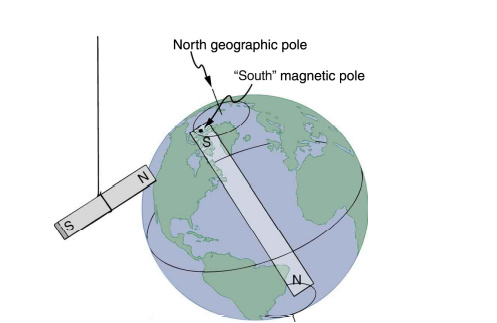
\includegraphics[scale=1.0]{img/earth_magnetic_field.png}\newpage
	As we have seen earlier, we can not separate the poles of a magnet. North and south poles always occur in pairs. Attempts to separate them will result in more pairs of poles. If we continue to split the	magnet, we will eventually get down to an atom with a north pole and a south pole—these, too, cannot be separated. The fact that magnetic poles always occur in pairs of north and south is true from the very large scale—for example, sunspots	always occur in pairs that are north and south magnetic poles—all the way down to the very small scale. Magnetic atoms have both a north pole and a south pole, as do many types of subatomic particles, such as electrons, protons, and neutrons.
	\newline 
	%	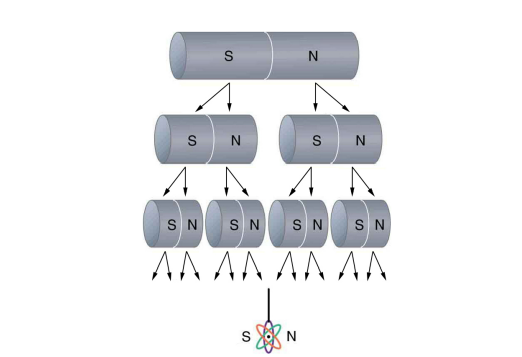
\includegraphics[scale=1.0]{img/sn_poles.png}\newline \newline
	\subsection*{Magnetic Field, Force and Sources}
	We have said earlier that magnetic force is a non-contact force and that it acts over a field. To visualize a magnetic field, we use hypothetical field lines that show how the magnetic force acts over the space. Here is an example of a magnetic field acting on iron fillings.\newline
	%	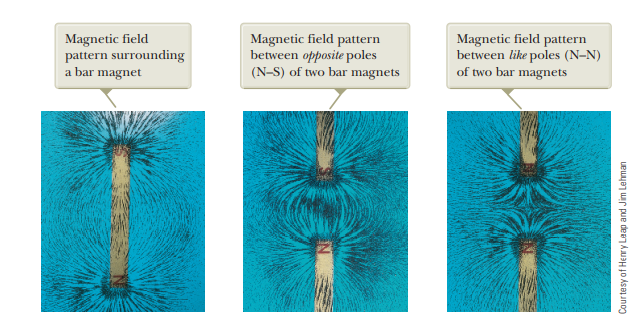
\includegraphics[scale=1.0]{img/magnetic_field_patterns.png}\newline \newline
	There are multiple sources of magnetic field. A straight current carrying wire is one prime example of a source of magnetic field. The magnetic field generated by a straight current carrying wire is determined by the \textbf{Right Hand Rule}. The basic idea in this rule is to align your thumb with the direction of current(\textbf{I}). Then, the direction in which the rest of your fingers curl show the direction of the magnetic field(\textbf{B}).
	
	
\end{document}	